\documentclass[a4paper,12pt]{article}
\usepackage{multimedia}
%% packages


\usepackage{braket}%braketnotationpackage

%% Theme
\usetheme{Berkeley} % theme for slides
%\usetheme{Frankfurt}
%\usetheme{Madrid}

%% Colors
%\usecolortheme{rose} % color for slides
\usecolortheme{beetle}
\definecolor{c1}{rgb}{0.5,0.5,0.5} % some green
\definecolor{c2}{rgb}{0.2,0.9,0.1} % some gray
%% see http://www.sharelatex.com/learn/Beamer
%\setbeamercolor*{palette primary}{fg=white,bg=c1} % upper part
%\setbeamercolor*{palette secondary}{bg=c2} % left part (background)
%\setbeamercolor*{sidebar left}{fg=white,bg=c1} % left part with links
%\setbeamerfont{section number projected}{ % section numbers
%  family=\rmfamily,
%  series=\bfseries,
%  size=\normalsize
%  }
%\setbeamercolor{section number projected}{bg=c1} % color of section numbers and others (fg: Fontm, bg:Hintergrund)
%\setbeamercolor{item projected}{bg=c1}
%\setbeamercolor{itemize item}{fg=c1}
%\setbeamercolor{author in sidebar}{fg=white}
%\setbeamercolor{footlinecolor}{fg=black,bg=c2}

%% Fonts
\usefonttheme{professionalfonts} % changes fonts

%% Foot
\usenavigationsymbolstemplate{} % deafult controls off
\setbeamertemplate{footline}[frame number] % slide number at the bottom
%\setbeamertemplate{footline}
%{%
%	\leavevmode%
%	\hbox{%
%	\begin{beamercolorbox}[wd=.3\paperwidth,ht=5ex,dp=1.5ex,left,leftskip=2mm]{footlinecolor}%
%		Foot information on the left over several lines
%	\end{beamercolorbox}%
%	\begin{beamercolorbox}[wd=.5\paperwidth,ht=5ex,dp=1.5ex,left,leftskip=2mm]{footlinecolor}%
%		Next foot part
%	\end{beamercolorbox}%
%	\begin{beamercolorbox}[wd=.2\paperwidth,ht=5ex,dp=1.5ex,right,rightskip=2mm]{footlinecolor}%
%		\insertframenumber{} / \inserttotalframenumber%
%	\end{beamercolorbox}%
%	}%
%	\vskip0pt%
%}
%% own commands
%\newcommand{\tbi}[1]{\textbf{\textit{#1}}}
\newcommand{\cm}[1]{{\tt \textcolor{orange}{#1}}}
\newcommand{\wl}[2]{\href{#2}{\textcolor{blue}{#1}}}
\newcommand{\att}[2]{\href{#2}{\textcolor{blue}{#1}}}
\newcommand{\imp}[1]{\underline{\textit{#1}}}

%%%%%%%%%%%%%%%%%%%%%%%%%%%%%%%%%%%%%%%%%%%%%%%%%%%%%%%%%%%
\begin{document}
\pagestyle{empty}
\title{Statistical Mechanics from Quantum Thermodynamics}
\author{Stefanopoulos Dimitris}
\date{\today}
\maketitle
\pagestyle{plain}

\section{Introduction} \par  As you can read in any article that discusses some aspect of quantum thermodynamics, it is emphasized that Quantum Thermodynamics is a broad interdisciplinary field. This is actually very accurate. From non-equilibrium statistical mechanics to quantum thermal machines a lot of different fields of physics use their various tools to study these "new" types of systems. \par However, the most additions into Q-Thermo have been done by Quantum Information Theory and this is not a surprise. In essence, thermodynamic systems are usually treated as open subsystems of a larger closed system. This idea is inherent in Quantum Mechanics in general, but it is essential in many sub-fields of Quantum Information Theory such as error-correction. Hence, I try to introduce the reader to a small fraction of Quantum Thermodynamics that may be to the interest of Statistical Mechanics. Specifically, this is a small semester project regarding a graduate level Statistical Mechanics course. Hopefully, the reader would find the subject matter intriguing.
\section{Foundations of Statistical Mechanics}\par
One of the issues that comes up when discussing the foundations of statistical mechanics is the apparent contradiction with quantum mechanics. At first site this phrase looks ridiculous since Quantum Mechanics have been used in Statistical Mechanics. In fact, some of our highly successful results such as Electron Gas, Bose-Einstein condensation, White Dwarf degenerate gas are based upon our knowledge of quantum mechanics. However,this is not entirely accurate.
\par  We need to emphasize that there is a conceptual ambiguity here. Indeed, we have used some results of quantum mechanics such as the discrete levels of energy and the spin of the particles. These are result of the Schr\"odinger
equation. Schr\"odinger's equation is just one of the postulates of quantum mechanics and let alone could be interpreted as a dynamical wave equation. Hence, from our treatment of quantum 
statistical mechanics we can see that it misses almost every property of the Hilbert Space. One can wonder, how on earth without using amplitudes derived from the Hilbert Space(the fundamental structure of a quantum system) we can end up with statistical properties that are valid? After all the postulate of \textit{a priori probability} is obviously inconsistent with the probabilities we derive by doing quantum mechanics.\par
There is a second argument regarding the apparent inconsistency of Quantum Mechanics and Statistical Mechanics. Dynamics of quantum theory is unitary. But, in statistical mechanics unitarity is somewhat ignored. Of course, in most cases Statistical Mechanics is studied in equilibrium thus talking about dynamics would become irrelevant. Still though, if we derive Thermodynamics from Statistical Mechanics we better include unitary evolution. In \cite{goold2016role} the issue is addressed in detail.
\section{Building the Thermal State}
The goal of building statistical mechanics from quantum thermodynamics can be defined clearly as the problem of using quantum mechanics to end up with thermal states. Thermal states as defined in \cite{PATHRIA2011115},\cite{potts2019introduction}.
\begin{equation}\hat{\tau}_{\beta, \mu}=\frac{e^{-\beta(\hat{H}-\mu \hat{N})}}{Z}
\label{thermal}
\end{equation}
with
\begin{equation}
Z=\operatorname{Tr}\left\{e^{-\beta(\hat{H}-\mu \hat{N})}\right\}
\end{equation}
Of course the above statements are about the grand canonical ensemble. Similarly, we can define the canonical ensemble. We conclude, an appropriate statement of the problem, would be to ask for a density matrix, meaning a quantum state that is equal to \eqref{thermal}. Rigorous proofs are a subject of current research. We will discuss here some partly successful approaches.
\section{First Step: Approach through typicality}
As always we consider the "thermal bath" as the universe and a subset of the universe as our system. We assume that the universe is in a pure state i.e. we have no ignorance about its quantum state. As an immediate result the state of the system could be in a mixed state. Intuitively even if we have no lack of knowledge about the state of the universe we still have "objective" lack of knowledge about the state of the system. Hence from the universal entropy zero we get some "local entropy" non zero. \par
Let us now to write down the concepts with a bit more clarity. Let $\mathcal{H}_{E}$ and $\mathcal{H}_{S}$ 
be the Hilbert space of the environment and the system respectively. Unavoidably, the Hilbert space of the universe would be: $\mathcal{H}_{E}\otimes \mathcal{H}_{S}$. In addition, let us assume that we impose an arbitrary universal constrain. This constrain can be about anything e.g. constant energy, constant number of particles or anything else you can imagine. This restriction forces the universe to a sub-space that satisfies condition $R$. Hence our system lives in a Hilbert space like:
\begin{equation}\mathcal{H}_{R} \subseteq \mathcal{H}_{S} \otimes \mathcal{H}_{E}
\end{equation}

Of course similarly with statistical mechanics, we assume that the dimension of the environment is much larger than that of the system. Let us now to define the maximally mixed state of the achievable universe $\mathcal{R}$ 
\begin{equation}
\mathcal{E}_{R}=\frac{\mathbb{I}_{R}}{d_{R}}
\label{equiprob}
\end{equation}
This is assumption consistent with the conventional a priori equal probability axiom. We also define the canonical state of the system when the universe is in its equiprobable mixed state:
\begin{equation}\Omega_{S}=\operatorname{Tr}_{E}\left(\mathcal{E}_{R}\right)
\end{equation}
Now what is shown in \cite{popescu2006entanglement} is that taking the universe to be in a pure state is not that far from taking it to be at \eqref{equiprob}. That is: for almost every pure state of
the universe, the system behaves as if it were in the equiprobable mixed state $\mathcal{E}_{R}$. The proof is technical and it is not in the scope of this essay. However, a qualitative description is possible.
\par There two very important notions that connect the above assumptions with Statistical Mechanics. Levy's Lemma and Typicality. A few words before we jump into the example. Levy's Lemma states that when a point $\textbf{P}=(p_1,p_2,p_3...)$ is selected at random from a hypersphere of high dimension
and $f(\textbf{P})$ does not vary too rapidly, then $f(\textbf{P}) \approx\langle f\rangle$ with
high probability. It is a manifestation of the law of large numbers in higher dimension. See \cite{milman2009asymptotic}.
\par
Along similar lines the concept of typicality argues that when you have a set of microstates $\textbf{X}$(as we have used as "the universe") under some constrain(as we have used $R$) that allows the system to be only in a subspace of its totality, trying to calculate the mean of an observable quantity $f(\textbf{X})$ will naturally end up to the mean of $f(\textbf{X})$ if it had no constrain R. Specifically if the mean is defined:
\begin{equation}
E_R[f]=\int_{R} f(\textbf{X}) d \mu
\end{equation}
and the variance as:
\begin{equation}\mathrm{V}_{\mathrm{R}}[f] \equiv \mathrm{E}_{\mathrm{R}}\left[\left(f-\mathrm{E}_{\mathrm{R}}[f]\right)^{2}\right]=\mathrm{E}_{\mathrm{R}}\left[f^{2}\right]-\mathrm{E}_{\mathrm{R}}^{2}[f]
\end{equation}
then when 
\begin{equation}\mathrm{V}_{\mathrm{R}}^{\frac{1}{2}}[f] \ll f_{\max }-f_{\min }
\end{equation}
$E_R$ is the typical $E$ and $E_R \approx E$. $f_{max}, f_{min}$ are the extremal values of $f$ under $R$. Of course this can be generalized into vectorial and tensorial observables. In our case the measure $\mu$ is motivated by the trace norm $\|M\|=\operatorname{Tr}|M|=\operatorname{Tr} \sqrt{M^{\dagger} M}$ but is not used directly. Trace norm of course represents a measure between quantum states $M=||\rho-\sigma||$($\rho$ and $\sigma$ are arbitrary density matrices).\par
In \cite{popescu2006entanglement} the authors among other things, they prove a theorem that they directly use in the following application in spin chains. The theorem states: 
\begin{theorem}
\label{theorem}
For a randomly chosen state $|\phi\rangle \in \mathcal{H}_{R} \subseteq$ $\mathcal{H}_{S} \otimes \mathcal{H}_{E}$ and arbitrary $\epsilon>0,$ the distance between the reduced density matrix of the system $\rho_{S}=\operatorname{Tr}(|\phi\rangle\langle\phi|)$ and
the canonical state $\Omega_{S}=\operatorname{Tr} \mathcal{E}_{R}$ is given probabilistically
$b y$
\[
\operatorname{Prob}\left[\left\|\rho_{S}-\Omega_{S}\right\| \geq \eta\right] \leq \eta^{\prime}
\]
where
\[
\begin{aligned}
\eta &=\epsilon+\sqrt{\frac{d_{S}}{d_{E}^{\mathrm{eff}}}} \\
\eta^{\prime} &=2 \exp \left(-C d_{R} \epsilon^{2}\right)
\end{aligned}
\]
In these expressions, $C$ is a positive constant (given by $\left.C=(18 \pi^{3}\right)^{-1}$),$d_{S}$ and $d_{R}$ are the dimensions of $\mathcal{H}_{S}$ and $\mathcal{H}_{R}$ respectively, and $d_{E}^{\text {eff }}$ is a measure of the effective size of the environment, given by
\[
d_{E}^{\mathrm{eff}}=\frac{1}{\operatorname{Tr} \Omega_{E}^{2}} \geq \frac{d_{R}}{d_{S}}
\]
where $\Omega_{E}=\operatorname{Tr}_{S} \mathcal{E}_{R} .$ Both $\eta$ and $\eta^{\prime}$ will be small quantities, and thus the state will be close to the canonical state
with high probability, whenever $d_{E}^{\text {eff }} \gg d_{S}$ (i.e. the effec-
tive dimension of the environment is much larger than that of the system) and $d_{R} \epsilon^{2} \gg 1 \gg \epsilon .$ This latter condition can be ensured when $d_{R} \gg 1$ (i.e. the total accessible
space is large), by choosing $\epsilon=d_{R}^{-1 / 3}$.
\end{theorem}
To demonstrate the techniques and the similarity with established statistical mechanics, instead of copying proofs and theorems we present this $1/2$ spin chain application from \cite{popescu2006entanglement}.
\par Let's define the Hamiltonian of the system under an external field in the $+z$ direction:
\begin{equation}
H=-\sum_{i=1}^{n} \frac{B}{2} \sigma_{z}^{(i)}
\end{equation}
We assume that we have $k$ spins as the system, hence $n-k$ spins form the environment. Now, we consider a restriction to one of these degenerate subspaces $\mathcal{H}_{R} \in \mathcal{H}_{S} \otimes \mathcal{H}_{E}$ in which $n p$ spins are in the excited state $\ket{1}$ (opposite to the field) and the remaining $n(1-p)$ spins are in the ground state
$\ket{0}$ (aligned with the field). In this case:
\begin{equation}
d_{S}=2^k \quad , \quad
d_{R}=\left(\begin{array}{c}
n \\
n p
\end{array}\right)
\end{equation}
in which for $d_{R}$ we enumerate all indistinguishable combinations in $\ket{1}$. Now using the above theorem we can prove that
\begin{equation}
\left\|\rho_{S}-\Omega_{S}\right\| \approx 0
\end{equation}
for sufficiently large $n \gg k$. Here of course $\Omega_{S}$ denotes the canonical state which is a standard statistical mechanics formula:
\begin{equation}
\Omega_{S}=(1-p)^{k} \sum_{s} \exp \left(-\frac{|s| B}{\mathrm{k}_{B} T}\right)|s\rangle\langle s|
\propto \exp \left(-\frac{H_{S}}{\mathrm{k}_{B} T}\right)
\label{Omega}
\end{equation}
One can readily see the similarities with \eqref{thermal} in the more formal quantum mechanical setting of density operators. Of course \eqref{Omega} is less general than \eqref{thermal}. All of the above results(the canonical ensemble formula from typicality) were originally motivated by \cite{goldstein2006canonical}

\section{Entanglement and Envariance}
Do no let the title plant the idea that the first road that derives the Canonical State does not include entanglement. In fact as we know even for just a couple of qubits $A$ and $B$ the Hilbert Space $\mathcal{H}_A \otimes \mathcal{H}_B$ has as members states that cannot be written as $\ket{A} \otimes \ket{B}$. This is obviously generalized in more qubits and more dimensions. In fact, in our theoretic approach of the universe as a single quantum entity, unavoidably we create the possibility of entangled states between the environment and the system ($\mathcal{H}_E \otimes \mathcal{H}_S $).
\begin{center}
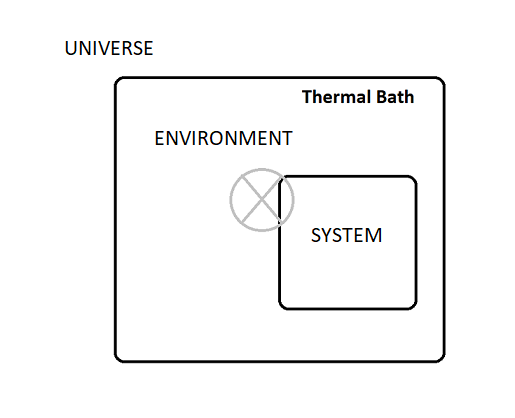
\includegraphics{figures/photo}
\end{center}
\par
So for this different entanglement approach we will just state the property of "envariance" upon which it is based. The reason that we won't further analyze their results is that this approach has raised a lot of critique in the latest years, specifically in \cite{alicki2015comments}. The author accuses for lots of ill-defined terms and I believe that most readers will tend to agree with him if they read both papers. However, the approach of envariance in \cite{deffner2016foundations} has been used by the same authors to derive Born's rule \cite{zurek2003environment}, hence it is not in any way ignorable. Although again there is some critique, see \cite{schlosshauer2003zurek} as an example.
\par
Let us describe the property of envariance. To do that we turn back to the standard vector quantum state and away from the density matrix formalism(of course the results are provable in any case). Think as usual the quantum system and its environment
as $\ket{\psi_{SE}}$ belonging in
$\mathcal{H}_S \otimes \mathcal{H}_E$. Then $\psi_{SE}$ is called envariant under a unitary map $U_{\mathcal{S}}=u_{S} \otimes \mathbb{I}_{E}$ iff there exists another unitary $U_{E}= \mathbb{I}_{E} \otimes u_{E} $ such that:
\begin{equation}
\begin{array}{l}
U_{S}\left|\psi_{S E}\right\rangle=\left(u_{S} \otimes \mathbb{I}_{E}\right)\left|\psi_{S E}\right\rangle=\left|\eta_{S E}\right\rangle \\
U_{E}\left|\eta_{S \mathcal{E}}\right\rangle=\left(\mathbb{I}_{S} \otimes u_{E}\right)\left|\eta_{S E}\right\rangle=\left|\psi_{S E}\right\rangle
\end{array}
\end{equation}
To illustrate the above we state a simple example. Let $\mathcal{S}$ and $E$ be two level systems and assume that $\left|\psi_{SE}\right\rangle \propto|\uparrow\rangle_{S} \otimes|\uparrow\rangle_{E}+|\downarrow\rangle_{S} \otimes|\downarrow\rangle_{E}$. Let's see the action of our operators now:
\begin{equation}
|\uparrow\rangle_{\mathcal{S}} \otimes|\uparrow\rangle_{E}+|\downarrow\rangle_{\mathcal{S}} \otimes|\downarrow\rangle_{E} \stackrel{U_{\mathcal{S}}}{\longrightarrow}|\downarrow\rangle_{\mathcal{S}} \otimes|\uparrow\rangle_{E}+|\uparrow\rangle_{\mathcal{S}} \otimes|\downarrow\rangle_{E}
\end{equation}
\begin{equation}
|\downarrow\rangle_{\mathcal{S}} \otimes|\uparrow\rangle_{E}+|\uparrow\rangle_{\mathcal{S}} \otimes|\downarrow\rangle_{E} \stackrel{U_{E}}{\longrightarrow}|\downarrow\rangle_{\mathcal{S}} \otimes|\downarrow\rangle_{E}+|\uparrow\rangle_{\mathcal{S}} \otimes|\uparrow\rangle_{E}
\end{equation}
From the above formulas it is obvious that we circle back to the original state but with exchanging amplitudes. Since the operations are Unitary the amplitudes must be equal. Obviously this property can extend to more complicated systems and it has been used by many authors for certain modern new approaches into Quantum Thermodynamics some of which we will discuss in the following section. 
\par As a final note, in \cite{vermeyden2015experimental} is reported experimental evidence of envariance. Thus, even a small change of these type of approaches being successful, emphasizes the importance of exploring them.
\section{State of the Art}
\subsection*{Information Theoretic Statistical Mechanics}
In this innovative paper \cite{chiribella2016entanglement}, the authors try to axiomatize statistical mechanics using four axioms motivated from information theory. The framework they use is called generalized probabilistic theory and it can be applied in principal to arbitrary physical theories. The axioms include very basic assumptions such as causality and purification.
\subsection*{Maxwell's Demon and Work done by a single molecule}
There is a triplet of papers/books written in modern Quantum Thermodynamics connections with Information Theory that describe the literature in Quantum Work,Information and their applications \citep{deffner2019quantum},\citep{vinjanampathy2016quantum},\citep{goold2016role}. Maxwell's demon is the well known creature that can separate fast moving particles form slow ones. In the quantum treatment the act of measurement is similar to copying the single bit information
about where the particle is to the Demon’s memory. Hence the work done by the Demon, and the information that is copied to the Demon's memory (or the process of erasure of its memory) must be somehow conceptually consistent with the quantum thermodynamic view. One of the goals is to define work as a purely quantum mechanical idea. Great work in this area has already been done an is still a subject of research.
\subsection*{Entropies:Thermo or Info?}
This is a long lived subject in Physics of Information. It tries to clarify the connections between thermodynamic and informational(statistical) entropies. Despite again for the incredible work that has been done from Quantum Information Theorists defining Quantum Entropies, many people are not satisfied by the possible narratives. Quantum Thermodynamic Research attempts to tackle these issues and resolve them.
\subsection*{Applications: Quantum Engines, Quantum Batteries}
Even though most of the work done in the field is about conceptual and somewhat philosophical implications, it would not be of much use if it had nothing to do with practical applications. The most understood ones that are a subject of theoretical and experimental research are Quantum Engines and Quantum Batteries. Quantum Thermal Engines is where people trying to interpret Temperature, Volume and Pressure quantumly. They use known cycles like Otto's, Carnot's and try to reproduce them for a quantum system in a way that makes sense.\par Quantum Batteries are self-explanatory. It has been hypothesized that an ideal quantum battery would require no recharge, since as a quantum system it could have a lifetime much larger than ours. Of course there are a lot of engineering issues that need to be resolved. Worth noting IBM's interest in this area of research, demonstrating the strong belief in the existence of marketable quantum batteries.


\section{Conclusions}
Most authors if not all, are agreeing to an important assumption. If we are going to view thermodynamic systems purely  from the quantum mechanical perspective, entanglement will play a huge role in our treatment. This cannot be though that surprising today. Quantum Information Theorists consider every subsystem coupled with other subsystems of the universe. Even spacetime is viewed these days as emergent from entanglement(famously Susskind has talked a lot about that).
In any case, the belief today is that Statistical Mechanics(together with Quantum Thermodynamics) is a an extremely successful theory of physics and it needs well-defined foundations based on Quantum Mechanics and Quantum Information Theory, with entanglement playing the vital role in our intuitions.



\bibliographystyle{abbrv}
\bibliography{bibliography/biblio}
\end{document}